%% GPW2026 本論文 (最終原稿) 下書き
%% 学会配布の jsample-gpw.tex をベースに、UTF-8 版 ipsj.cls (v4.1) で組む構成
%% Overleaf では latexmkrc により platex + pbibtex + dvipdfmx でコンパイルされる
%% 書き方の約束 (太字を使わない等) は OUTLINE.md の「書き方の約束」
\documentclass[submit]{ipsj}
% [submit] をつけないとフォントの問題が起きる可能性がある (GPWサンプルの注記)

% 受付日などを消す
\makeatletter
\def\@uketsuke{}
\def\@euketsuke{}
\def\SHUBETUname{}
\makeatother

% ページ番号を消す
\pagestyle{empty}

\usepackage[dvipdfmx]{graphicx}
\usepackage{latexsym}
\usepackage{amsmath,amssymb}
\usepackage{url}
%\usepackage{times,mathptmx} % お好みで

% TODO: タイトルは主張の軸 (性能=価値スクリーン / 表現=クラスタ) が決まってから確定する
\title{デジタルカーリングにおけるMCTS候補手削減のための\\価値考慮型クラスタリングの適用}
% 英文タイトル・英文概要は一旦省略 (2026-10-16 ユーザー指示). 追加するときは下の \etitle と eabstract/ekeyword を戻す
%\etitle{English Title}

% TODO: 所属の表記 (研究科名・住所を載せるか) を確認
\affiliate{MU}{明治大学\\
Meiji University}

\author{仲 亜斗夢}{Atomu Naka}{MU}[ce265004@meiji.ac.jp]
\author{横山 大作}{Daisaku Yokoyama}{MU}[dyokoyama@meiji.ac.jp]

\begin{document}

\begin{abstract}
和文概要．
\end{abstract}
% '22年以後 日英キーワードを加えて統一した方が良い (GPWサンプルの注記)
\begin{jkeyword}
デジタルカーリング，モンテカルロ木探索，クラスタリング
\end{jkeyword}

%\begin{eabstract}
%English abstract.
%\end{eabstract}
%\begin{ekeyword}
%Digital Curling, Monte Carlo Tree Search, Clustering
%\end{ekeyword}

\maketitle
% ページ番号を消す
\thispagestyle{empty}

%======================================================================
\section{はじめに}
\label{sec:intro}
% このセクションでは、この論文全体を通しての目的と結果が分かるように書きます。また、この論文で必要となる一般的に知られていない前提知識（デジタルカーリングとは）についても詳しく書きます。そして、そのテーマが抱える課題点に対して、この論文ではどんな手法でアプローチして、どういう結果が得られたのかを書きます。

カーリングは，氷上で石（ストーン）を滑らせ，ハウスと呼ばれる同心円の的の中心（ティー）にどれだけ近づけられるかを競う競技である．
「氷上のチェス」と呼ばれるように，数手先の石の配置を見越した読みが要求される．
デジタルカーリング~\cite{dc3}は，この競技を2次元の物理シミュレータ上で再現した対戦環境であり，
モンテカルロ木探索（MCTS）を中心とした思考エンジンが研究されてきた~\cite{owatari2016,kato2016,yee2016}．

試合は複数のエンドからなり，各エンドでは2チームが交互に8投ずつ，計16投を投げる．
エンドの終わりに，ティーに最も近い石（No.1ストーン）を持つチームが，相手チームの最もティーに近い石より内側にある自チームの石の数だけ得点する．
得点に数えるのはハウスの中の石だけである．
エンドの最終投を投げる後攻は，最後に石の配置を変えられるため有利である．
主なショットには，狙った位置に石を止めるドロー，他の石に当てて動かすヒット，相手の石に密着させて止めるフリーズ，
ハウスの手前に石を置いて後ろの石を守るガードがある．
ガードのうち，ハウスの中の自分の石の前に置くものをポストガード，ハウスの手前の決まった位置に置くものをプレガードと呼ぶ．
また，自分の石に当ててティーの方へ押し込むヒットをレイズと呼ぶ．
デジタルカーリングでは，プレイヤは1投ごとに石の初速$(v_x, v_y)$と回転方向（時計回りか反時計回り）を選ぶ．
行動は連続値であり，さらに初速には正規分布に従う誤差（以下，外乱）が加わるため，狙いどおりに投げても結果は確率的に変わる．

連続行動空間でMCTSを用いる際には，ドロー，ヒット，ガードなどの候補手を有限個生成し，それを木の分岐とすることが多い．
しかし候補手を十分に用意すると分枝数が大きくなり（本論文の設定では1局面あたり33〜153手），
限られた計算予算のもとでは1つの候補手に割り当てられるシミュレーション回数が不足する．
% 出典: test_positions500 の候補数 N (平均 70.6, 中央値 61)
対戦では持ち時間が決まっているため，少ない計算量で良い手を選べることは実用上も重要である．
大きな行動空間や連続行動空間でのMCTSについては，
ボロノイ分割に基づいて行動をサンプリングするVOOT~\cite{kim2020voot}や，
学習した遷移モデルから状態ごとに不要な行動を除く状態条件付き行動抽象化~\cite{kwak2024}
などが提案されている（\ref{sec:related}章）．

われわれの先行研究~\cite{naka_gi58}では，各候補手を打った後の盤面（以下，結果盤面）に階層的クラスタリングを適用し，
各クラスタの代表手のみを探索対象に残すことで候補手を削減する手法を提案した．
結果盤面でクラスタリングするのは，外乱のあるカーリングでは「どこを狙ったか」よりも
「その手がどのような盤面を引き起こすか」によって手の役割が決まると考えたためである．
本論文では，この手法をMCTSに拡張したものをClusterMedoidと呼び，既存手法として扱う．
ClusterMedoidは，各クラスタの代表手として盤面上で最も中心的な候補（medoid）を選ぶが，
この選び方は手の得点期待値を考慮していないため，代表手が有望な手になるとは限らない．
また先行研究では，全候補を探索する手法が選んだ手との一致率で性能を評価していたが，
計算予算が限られた全探索の選択は正解の代わりにならないという問題もあった．

そこで本論文では，結果盤面によるクラスタは保ったまま，
クラスタの採用と代表手の選出に得点期待値を用いる手法ClusterValueを提案する．
ClusterValueは，各候補手の得点期待値を少数のロールアウトで安価に推定し，
その平均値（クラスタ価値）が高い上位のクラスタから，それぞれ推定値が最大の候補を代表手として探索木に残す．
さらに，木の中で手を評価するたびに外乱ありで打ち直す外乱込み評価を組み合わせ，
「狙った結果」ではなく「その手を試みる価値」を評価する．

性能は，各候補手を外乱ありで200回ロールアウトして求めた得点期待値（以下，審判値）を正解の基準とし，
選んだ手と最良手との審判値の差（regret）で評価した．
層化抽出した500局面で，物理シミュレーションの回数を揃えた等予算の条件で比較した結果，
提案手法は既存手法ClusterMedoidよりregretが22\%小さく，候補を絞らない全探索も有意に上回った．
その利得は計算予算が小さいほど大きかった．
% 出典: gpw_experiment/paper_numbers/numbers.txt (500局面 x 5seed, P=200) A9P5N 0.309 / A1N 0.334 / A2N 0.396
さらに，結果盤面のクラスタが人間にとって意味のある単位になることを，盤面の図を用いて示した．
クラスタは手を結果の種類でまとめ，相手の中心の石を取り除くような他と似ていない最良手や，
即時の得点は低いがエンド全体では同等に有利な別の手を，それぞれ独立したまとまりとして示す．
また，結果盤面による分割は，VOOTのような行動空間の分割よりも価値のまとまった領域を作ることを示した．

本論文の構成は次のとおりである．
\ref{sec:related}章で関連研究を述べ，\ref{sec:method}章で既存手法と提案手法を説明する．
\ref{sec:exp}章で性能の比較実験を，\ref{sec:discussion}章で既存手法との差とクラスタの視覚的評価についての考察を述べ，
\ref{sec:future}章で今後の課題を述べる．

%======================================================================
\section{関連研究}
\label{sec:related}
% このセクションは論文の最後の仕上げの直前に書きます。内容はまだ未定で大丈夫です。ただ、触れる予定のあるテーマだけをサブセクションとして記しておくといいです。
% (2026-10-18) 本文は以前の下書きのまま. 参照先の節番号だけ新しい構成に合わせた. 最後の仕上げで書き直す.

\subsection{デジタルカーリングの思考エンジン}
\label{sec:related-curling}

デジタルカーリングでは，候補手を有限個に絞ったうえで探索する手法が主に研究されてきた．
大渡ら~\cite{owatari2016}は，MCTSに基づく思考エンジン「歩」を開発した．
歩は，ドロー，ヒット，フリーズ，ガードなどのショットの種類ごとに盤面に応じた候補手を生成し，
UCB1によって有望な候補手に多くのプレイアウトを配分する．
本論文の候補手生成も，歩の候補手生成を参考にしている．
% 実装: src/shot_generator generatePool (歩相当. ComeAround/Peel 等は未生成; experiments/REINVESTMENT_EXPERIMENT_GUIDE.md)
加藤ら~\cite{kato2016}は，行動空間をグリッドで離散化し，不確定性を考慮したExpectimax探索を行った．
いずれの手法でも1局面あたりの候補手は多く，探索を深くするうえでの障害となっていた．

Yeeら~\cite{yee2016}は，カーリングのシミュレータを対象に，実行時の誤差のモデルをカーネルとするカーネル回帰によって，
行動の価値の推定を周辺の行動へ汎化するKR-UCTを提案した．
KR-UCTは，ある行動の試行で得られた結果を近い行動の評価にも用い，初期の候補手の外側にある行動も探索する．
Leeら~\cite{lee2018curling}は，カーネル回帰による連続行動の木探索を深層ニューラルネットワークと組み合わせ，
教師あり学習と自己対戦による強化学習でデジタルカーリングのプログラムを構築した．
KR-UCTが行動のパラメータ空間での近さによって情報を共有するのに対し，本論文は結果盤面の近さによって候補手をまとめる．
そのため，回転方向が異なり行動のパラメータとしては離れた2つのドローでも，同じ位置に止まれば同じクラスタに入りうる．
またYeeらは，良い手を含めるために候補を増やすことと，有望な候補を正確に評価することの間にトレードオフがあると指摘している．
\ref{sec:res-budget}節で行うregretの分解は，このトレードオフを等予算の条件で定量化したものと位置づけられる．

\subsection{連続・大規模な行動空間でのMCTS}
\label{sec:related-continuous}

連続行動空間でのMCTSには，各ノードで「どの行動を試すか」を連続空間上の最適化の問題として扱う手法がある．
HOOT~\cite{mansley2011hoot}は，行動空間を階層的に分割しながら価値の高い領域に試行を集中させる連続腕バンディットのアルゴリズム（HOO）を，木の各ノードに適用した．

Kimら~\cite{kim2020voot}のVOOTは，木の各ノードで，ボロノイ分割に基づくブラックボックス最適化VOOによって行動をサンプリングする．
VOOは，それまでに評価した行動を母点とするボロノイ分割を用いる．
確率$\omega$では行動空間全体から一様に，すなわち各ボロノイセルの体積に比例してサンプリングし，
確率$1-\omega$では現在の最良の行動のボロノイセルの中からサンプリングする．
分割は陽に構成せず，母点との距離だけで扱えるため，高次元の行動空間にも適用できる．
VOOTは決定的な遷移をもつ高次元の連続行動の問題を対象とし，regretの上界も示されている．

本論文の手法は，候補を領域に分けて各領域を1つの代表で扱い，最良の候補を含む領域に探索を集中させる点で，VOOと共通する．
とくに，ClusterValueが推定値の最も高い候補の属するクラスタを必ず採用する規則（\ref{sec:method-select}節）は，
VOOが最良の行動のボロノイセルを重点的に探索することに対応する．
一方で，次の3点が異なる．
第一に，VOOは行動のパラメータ空間を行動どうしの距離で分割するが，本論文は結果盤面どうしの距離で候補手を分割する．
カーリングでは，わずかな狙いの違いで石に当たるかどうかが変わって結果が大きく変わる一方，
離れた行動が同じ結果を生むこともあるため，行動空間での近さは手の役割の近さを必ずしも意味しない．
第二に，VOOTは決定的な遷移を前提とするが，カーリングには外乱があり，同じ行動でも結果がばらつく．
本論文では，クラスタは外乱なしの結果盤面から作り，価値は外乱込みで評価することでこれに対処する（\ref{sec:method-noisy}節）．
第三に，VOOTは行動を新たに生成するのに対し，本論文は候補手生成器が作った有限個の候補から選別する．
両者は排他的ではなく，有望なクラスタの周辺で新たな候補を生成するといった組み合わせも考えられる．
この対応関係と，どちらの空間で分割するのがよいかは，\ref{sec:disc-voronoi}節で定量的に検討する．

また，確率的な遷移をもつ問題では，木のノードを状態ではなく行動の系列に対応させ，
プレイアウトのたびに遷移を標本化し直すopen-loop型の探索も用いられる~\cite{perez2015openloop}．
本論文の外乱込み評価（\ref{sec:method-noisy}節）は，この考え方を価値の評価に用いたものである．

\subsection{状態と行動の抽象化}
\label{sec:related-abstraction}

MCTSの分枝を減らす別の方向として，等価な状態や行動をまとめる抽象化がある．
Hostetlerら~\cite{hostetler2014}はMCTSにおける状態の集約を扱った．
ASAP-UCT~\cite{anand2015asap}は，抽象状態への遷移確率と即時コストが等しい状態行動対を等価とみなし，
等価な対どうしで木の価値の更新を共有する．
OGA-UCT~\cite{anand2016oga}は，この抽象化を探索の途中で逐次計算する．
これらは等価性が成り立つ状態や行動をまとめるものであるが，
石の位置が連続値であるカーリングでは，異なる手の結果盤面が厳密に一致することはほとんどない．

Kwakら~\cite{kwak2024}は，行動が複数の部分行動の組み合わせからなる問題を対象に，状態条件付き行動抽象化を提案した．
この手法は，潜在ダイナミクスモデルと補助ネットワークを学習して，現在の状態からの遷移に関係する部分行動を推定し，
木の各ノードで遷移に関係しない部分行動の探索を省くことで探索空間を縮小する．
本論文の手法も，ノードごとにその局面での行動の結果に基づいて行動をまとめる点で，状態条件付きの行動抽象化の一種とみなせる．
ただし，Kwakらが学習したモデルから遷移への寄与を推定するのに対し，本論文はシミュレータで得た結果盤面を直接用いるため，学習を必要としない．
また，Kwakらは決定的な遷移のもとで部分行動の単位で冗長性を判定するが，
本論文は外乱のある環境で，行動全体を結果盤面の近さに基づいて近似的にまとめる．

近似的な抽象化では，同じまとまりの中に価値の異なる行動が混在しうる．
本論文の結果は，このような場合には，まとまりの作り方に加えて，まとまりの中からどの行動を代表として残すかが性能を左右することを示している．
実際，medoidによる代表手の選出は無作為な選出と同等であり，
全探索を上回ったのは得点期待値に基づいてクラスタと代表手を選んだ場合であった（\ref{sec:res-repr}節）．
% 出典: E14/E16 (A2N≈A5N p=0.79, A9P5N 0.309 < A1N 0.334 < A2N 0.396)

%======================================================================
\section{提案手法}
\label{sec:method}
% このセクションではまず既存手法がどういうもので、今回提案する手法はどういうものなのかを説明する。それから、新たに追加したギミック（今回だと例えばmedoidの選び方を変えたとか、得点期待値の評価値を加えたとか、おおまかな説明をさらにサブセクションとして確立する。それでこのセクションを読めば提案手法がどんなものなのかが分かる。この後に続く実験セクションで読み手にこの提案手法がどのように評価されたのかを意識させる。）

本論文で扱う手法は，いずれもMCTSの各ノードで候補手生成器が$N$個の候補手$a_1,\dots,a_N$を生成し，
それぞれを外乱なしでシミュレーションして結果盤面$s_1,\dots,s_N$を求めたうえで，どの候補手を子として残すかだけが異なる．
既存手法ClusterMedoid（\ref{sec:method-medoid}節）は，結果盤面をクラスタリングし，各クラスタで盤面上最も中心的な候補を代表手として残す．
提案手法ClusterValue+Nは，同じクラスタを用いたまま，次の3点を変更する．
第一に，各候補手の得点期待値を少数のロールアウトで推定し，クラスタの価値を求める（\ref{sec:method-estimate}節）．
第二に，代表手をmedoidではなくクラスタ内で推定値が最大の候補とし，価値の高い上位のクラスタだけを子として残す（\ref{sec:method-select}節）．
第三に，木の中で手を評価するたびに外乱ありで打ち直す外乱込み評価を用いる（\ref{sec:method-noisy}節）．
既存手法との違いを\tabref{tab:diff}にまとめる．
\ref{sec:exp}章では，第三の変更の効果を\ref{sec:res-noisy}節で，第一と第二の変更の効果を\ref{sec:res-repr}節で検証し，
候補を絞ること自体の利得を全探索との比較によって\ref{sec:res-budget}節で検証する．

\begin{table}[tb]
\caption{既存手法ClusterMedoidと提案手法ClusterValue+Nの違い}
\ecaption{Differences between ClusterMedoid and ClusterValue+N.}
\label{tab:diff}
\centering
\begin{tabular}{p{0.2\columnwidth}p{0.32\columnwidth}p{0.32\columnwidth}}\hline\hline
 & ClusterMedoid & ClusterValue+N \\\hline
代表手の選び方 & medoid（盤面距離の総和が最小） & クラスタ内で推定値$\hat{e}_i$が最大 \\
採用するクラスタ & すべて & 価値の上位$K$個（最良候補のクラスタを必ず含む） \\
ルートの子の数 & $\lceil 0.2N \rceil$（平均14.4） & $\lfloor P/50 \rfloor$（$P=200$で4） \\
事前ロールアウト & なし & 各候補$R_{\mathrm{pre}}=5$回 \\
評価の規約 & 決定的 & 外乱込み \\\hline
\end{tabular}
\end{table}

\subsection{既存手法：ClusterMedoid}
\label{sec:method-medoid}

ClusterMedoidは，先行研究~\cite{naka_gi58}の候補削減をMCTSの各ノードに適用した手法である．
まず，結果盤面どうしの距離$d(s_i, s_j)$を，盤面の戦術的な違いを捉える次の8項目の重み付き和として定義する．
\begin{enumerate}
\setlength{\itemsep}{0pt}
\item 元の盤面にあった石の移動量の差
\item 投げた石の停止位置の差
\item 石の有無（場外に出たかどうか）の不一致
\item 石が属する領域（ハウス内，ガードゾーン，それ以外）の不一致
\item 既存の石に触れたかどうかの不一致
\item 投げた石と最も近い石との距離の差
\item その時点で数えた得点の差
\item No.1ストーンを持つチームの不一致
\end{enumerate}
% 実装: experiments/mcts_shared.cpp distDelta (重み 2/4/30/12/15/5/8/10)
% TODO: 重みを表で示すか，先行研究~\cite{naka_gi58}を参照するだけにするか決める
この距離に基づき，平均連結法による階層的クラスタリングで候補手を$K_c = \lceil rN \rceil$個のクラスタに分割する（$r=0.2$）．
各クラスタからは，クラスタ内の他の候補との距離の総和が最小となる候補（medoid）を代表手とし，
すべてのクラスタの代表手を子とする．
評価に用いた500局面では，ルートの子の数は平均14.4個であった．
% 出典: RESEARCH_OUTLINE §7 (N=33〜153, 平均 70.6, K=ceil(0.2N) の実測平均 14.4)

ClusterMedoidの代表手の選び方は，盤面の中心性のみに基づいており，手の得点期待値を考慮していない．
そのため，同じクラスタに得点期待値の高い候補と低い候補が混在する場合や，
得点期待値の低いクラスタが多数を占める場合には，有望でない手に探索予算が割かれる．
先行研究~\cite{naka_gi58}でも，代表点の選び方の改善と，大きなクラスタからの代表の選び方が課題として残されていた．

\subsection{得点期待値の推定とクラスタ価値}
\label{sec:method-estimate}

ClusterValueは，まず各候補手$a_i$について，その結果盤面からエンドの終わりまでのロールアウトを$R_{\mathrm{pre}}$回行い，
エンドの純得点の平均$\hat{e}_i$を求める．
候補手を打った時点でエンドが終わる場合は，そのエンドの得点をそのまま用いる．
次に，ClusterMedoidと同じ距離と手順で候補手を$K_c$個のクラスタ$C_1,\dots,C_{K_c}$に分割し，
各クラスタの価値（クラスタ価値）をメンバーの推定値の平均
\begin{equation}
v(C_c) = \frac{1}{|C_c|}\sum_{i \in C_c} \hat{e}_i
\label{eq:cluster-value}
\end{equation}
とする．
$R_{\mathrm{pre}}$は小さい（本論文では5回）ため，個々の候補の推定値はばらつきが大きい．
クラスタ単位で平均を取ることで，このばらつきを抑えたうえで，どの種類の結果が有望かを比較できる．
クラスタ価値の順位が個々の候補の推定値の順位より審判値の順位に近いことは，\ref{sec:disc-visual}節で示す．

\subsection{代表手とクラスタの選び方}
\label{sec:method-select}

ClusterValueは，クラスタをクラスタ価値の高い順に並べ，上位$K$個のクラスタから，それぞれ$\hat{e}_i$が最大の候補を代表手として子にする．
ただし，全候補の中で$\hat{e}_i$が最大の候補が属するクラスタは，価値の順位によらず必ず採用する．
クラスタ価値は平均であるため，有望な手が価値の低い手と同じクラスタにあるとそのクラスタの価値は低くなるが，
この規則によって推定値が最も高い手は必ず子に残る．
子の数$K$は，子1つあたりに確保したい訪問回数$V$を用いて$K=\max(1, \lfloor P/V \rfloor)$とする．
本論文では$V=50$とし，$P=200$のとき$K=4$である．
既存手法がすべてのクラスタの代表を子とするのに対し，提案手法は子を少数に絞り，その分だけ1つの子あたりの訪問回数を確保する．
この選び方はルートノードだけに適用し，深さ1以降のノードではClusterMedoidと同じ規則で子を作る．
% TODO: 深さ1以降を ClusterMedoid にした理由を書くか (事前ロールアウトのコスト / A10 は修正木で再評価していない)

\subsection{外乱込み評価}
\label{sec:method-noisy}

通常のMCTSの木は，外乱なしでシミュレーションした結果盤面を子の状態とする．
この決定的評価では，各手は「狙いどおりに投げられた場合」の価値で評価される．
一方，実際の対戦では手は外乱を伴って実行されるため，
わずかなずれで結果が大きく変わる手は，決定的評価では過大評価されやすい．
本論文で正解の基準とする審判値も，外乱ありで打ち直した結果の平均，すなわち「その手を試みる価値」である．

そこで外乱込み評価では，木の構造（候補手の生成，クラスタリング，候補の選別）は外乱なしの結果盤面から作ったまま，
価値の評価だけを外乱込みで行う．
具体的には，プレイアウトのたびに，選んだ手をその時点で到達している実際の盤面から外乱ありでシミュレーションし直し，
得られた盤面を次のノードへ運ぶ．
葉のロールアウトも，この外乱込みで到達した盤面から行う．
ClusterValueの事前推定（\ref{sec:method-estimate}節）でも，候補手を毎回外乱ありで打ち直してからロールアウトする．
これにより，各ノードの価値は「その手順を外乱のもとで試みたときの得点期待値」の推定となる．
これは，木のノードを行動の系列に対応させるopen-loop型の探索~\cite{perez2015openloop}の考え方を，価値の評価に用いたものである．
% 実装: --noisy-tree (experiments/reinvest_experiment.cpp runPlayout / estimateRootScores)

外乱込み評価は候補の選別方法とは独立であり，他の手法にも適用できる．
以下，外乱込み評価を適用した手法を「手法名+N」と表記する（例：AllGrid+N）．
本論文の提案手法は，ClusterValueに外乱込み評価を組み合わせたClusterValue+Nである．

%======================================================================
\section{実験}
\label{sec:exp}
% 実験目的が足りない書く。このセクションには、実験目的、比較手法、評価指標、実験条件、実験結果、をそれぞれサブ区セクションとして分けて書く。一番最後に実験全体を通しての提案手法に対する考察のサブセクションを書けばこのセクション全体がまとまって見える。提案手法と既存手法の違いを性能面で評価する。そのためには、このセクションでは評価に使われる審判値となにをしたのかを書いていく。今回の実験で書くことは、外乱を加えたらどうなるのか、全探索と比べてどういう場面だとクラスタリングの方が優れるのかのプレイアウト予算の変化、クラスタの代表手の選び方が提案手法と既存手法が異なるが、その影響はどうなのか、をまずは書きたい。図や表を積極的に出していく。

\subsection{実験の目的}
\label{sec:exp-purpose}

本実験の目的は，提案手法ClusterValue+Nの性能を，既存手法ClusterMedoidおよび候補を絞らない全探索と，計算予算を揃えた条件で比較することである．
とくに次の3点を明らかにする．
\begin{enumerate}
\setlength{\itemsep}{0pt}
\item 外乱込み評価を加えると，各手法の性能はどう変わるか（\ref{sec:res-noisy}節）
\item 全探索と比べて，どのような計算予算のときに候補を絞る方が優れるか（\ref{sec:res-budget}節）
\item 代表手の選び方（既存手法のmedoidと提案手法の得点期待値）の違いは，性能にどう影響するか（\ref{sec:res-repr}節）
\end{enumerate}
また，本実験で得たクラスタは，\ref{sec:disc-visual}節の視覚的評価にも用いる．

\subsection{比較手法}
\label{sec:exp-methods}

比較する手法は次の5つである．
\begin{itemize}
\setlength{\itemsep}{0pt}
\item AllGrid：全候補を子とする全探索．候補の取りこぼしはないが，ルートの子は平均70.6個になる．
\item ClusterMedoid：既存手法（\ref{sec:method-medoid}節）．ルートの子は$\lceil 0.2N \rceil$個（平均14.4個）．
\item ClusterValue：提案手法（\ref{sec:method-estimate}節，\ref{sec:method-select}節）．ルートの子は4個．
\item RandomK：ClusterMedoidと同じ数の候補を無作為に選んで子とする対照．
\item RandomK4：ClusterValueと同じ4個の候補を無作為に選んで子とする対照．
\end{itemize}
% 出典: test_positions500 の N の平均 70.6
RandomKはmedoidによる選び方を，RandomK4は得点期待値による選び方を，それぞれ同じ子の数の無作為な選び方と比べるための対照である．
各手法を決定的評価と外乱込み評価（+N）の両方で実行した．ただしRandomK4は外乱込み評価のみである．

\subsection{評価指標}
\label{sec:exp-metric}

正解の基準として，各局面の全候補手について，候補手を外乱ありで打ち直してからエンドの終わりまでロールアウトすることを200回繰り返し，
手番側から見たエンドの純得点の平均を求めた．これを審判値$q$と呼ぶ．
審判値は「その手を試みる価値」の推定であり，探索木を用いないため各手法の実装に依存しない．
手法が選んだ手$a$のregretを$q^{*}-q(a)$とする．ここで$q^{*}$は局面内の審判値の最大値であり，regretは小さいほど良い．
審判値の標準誤差は約0.10点であるが，1位と2位の候補の審判値の差は中央値で0.073点とこれより小さく，
約7割の局面では「どの手が最良か」自体が不安定である．
そのため，先行研究~\cite{naka_gi58}で用いた最良手との一致率ではなく，値の差であるregretで評価する．
% 出典: E06 (審判の監査)

さらにregretを，選別で最良手を落としたことによる損失（選別損失．$q^{*}$と，ルートの子に残った候補の審判値の最大値との差）と，
残りの損失（木の損失．子の中から最良のものを選べなかったことによる損失）の和に分けて分析する．

\subsection{実験条件}
\label{sec:exp-setup}

実験条件を\tabref{tab:settings}に示す．
評価局面は，歩の方策関数~\cite{owatari2016}を移植した方策どうしの自己対戦（序盤の数投は無作為に選択）から抽出した．
先頭の200局面は主に石の数と進行段階で層化して抽出し，残りの300局面は，盤面の型
（石が0〜1個，2〜4個，相手のNo.1ストーンを除去できる形，密着できる形，空きが多い形，石が6個以上）と進行段階で層化して抽出した．
このため，本論文で示す局面の割合は実戦での出現頻度とは異なる．
500局面のうち，エンドの最終投の局面は32局面（6.4\%）である．
% 出典: RESEARCH_OUTLINE §2.4 (test_positions500 = test_positions200 + pick_positions_stratified.py --seed 31),
%       局面のプール = experiments/generate_test_positions.cpp (gPolicy の自己対戦, 序盤 opening_random 手は乱択)

探索木は深さ3まで展開し，エンドの最終投を越える枝は終端としてそのエンドの得点を報酬とする．
ロールアウト方策は，各手番でハウスを覆う位置へのドロー，相手のNo.1ストーンへのヒットなど6〜10個の候補を生成し，
確率0.3で無作為に，それ以外は1投後の盤面で数えた得点が最大となる候補を選ぶ．
ロールアウトの投球は外乱ありでシミュレーションする．
% 実装: experiments/mcts_shared.cpp rolloutFromState (epsilon=0.3), ShotGenerator::generateRolloutCandidates
% 出典: extern/DigitalCurling3 player_normal_dist_factory.hpp (stddev_speed, stddev_angle の既定値)

予算はプレイアウト回数$P$で揃えた．
このとき1局面あたりの物理シミュレーション回数は，事前推定の分だけClusterValue+NがAllGrid+Nより3.6\%多い．
% 出典: RESEARCH_OUTLINE §2.5 (500局面, A9P5N 75.7k / A1N 73.1k)
本論文の比較はシミュレーション回数を揃えたものであり，実時間の比較ではない．
統計検定は，局面ごとに5シードのregretを平均して1つの値とし，
9条件（\tabref{tab:main}）のFriedman検定の後，全36対についてWilcoxonの符号順位検定を行い，Holm法で補正した~\cite{demsar2006}．
以下では補正後の$p$値を示す．
% 出典: scripts/gpw_paper_numbers.py -> gpw_experiment/paper_numbers/numbers.txt (Friedman p=4e-65)

\begin{table}[tb]
\caption{実験条件}
\ecaption{Experimental settings.}
\label{tab:settings}
\centering
\begin{tabular}{p{0.34\columnwidth}p{0.56\columnwidth}}\hline\hline
項目 & 設定 \\\hline
評価局面 & 自己対戦から層化抽出した500局面 \\
候補手の数$N$ & 1局面あたり33〜153手（平均70.6） \\
シミュレータ & デジタルカーリング~\cite{dc3} \\
外乱 & 初速の大きさと向きに正規分布の誤差（標準偏差0.0076\,m/s，0.0018\,rad） \\
探索の深さ & 3 \\
プレイアウト予算$P$ & 200（\ref{sec:res-budget}節では100〜800） \\
葉のロールアウト$R$ & 10回 \\
子の選択 & UCB1（各ノードの手番側の価値を最大化） \\
報酬 & 探索開始時の手番側から見たエンドの純得点 \\
最終的に選ぶ手 & ルートの子のうち訪問回数が最大の手 \\
クラスタ数$K_c$ & $\lceil 0.2N \rceil$ \\
事前推定$R_{\mathrm{pre}}$ & 5回（ClusterValueのみ） \\
ClusterValueの子の数$K$ & 4（$V=50$） \\
乱数のシード & 5通り \\\hline
\end{tabular}
\end{table}

\subsection{実験結果}
\label{sec:exp-results}

\subsubsection{全体の比較}
\label{sec:res-main}

\tabref{tab:main}に各手法のregretを示す．
外乱込み評価の条件では，提案手法ClusterValue+Nのregretが0.309と最も小さかった．
これは等予算の全探索AllGrid+N（0.334）より有意に小さく（$p=2\times10^{-4}$），
既存手法ClusterMedoid+N（0.396）より22\%小さい（$p=4\times10^{-8}$）．
局面単位では，ClusterValue+Nの方がregretが小さかった局面は，AllGrid+Nに対して297，ClusterMedoid+Nに対して282であり，
大きかった局面はそれぞれ198と205であった．
決定的評価の条件でも，ClusterValueはClusterMedoidより有意に小さく（0.423と0.488，$p=6\times10^{-4}$），
AllGrid（0.418）とは差がなかった（$p=1.0$）．
% 出典: gpw_experiment/paper_numbers/numbers.txt (局面単位の5seed平均で regret が小さい/大きい局面数)

\begin{table}[tb]
\caption{各手法のregret (500局面×5シードの平均，$P=200$．小さいほど良い)}
\ecaption{Regret of each method (500 positions $\times$ 5 seeds, $P=200$; lower is better).}
\label{tab:main}
\centering
\begin{tabular}{lcc}\hline\hline
手法 & 決定的評価 & 外乱込み評価（+N） \\\hline
AllGrid（全探索） & 0.418 & 0.334 \\
ClusterMedoid（既存手法） & 0.488 & 0.396 \\
RandomK（$\lceil 0.2N \rceil$個） & 0.491 & 0.383 \\
RandomK4（4個） & -- & 0.552 \\
ClusterValue（提案手法） & 0.423 & 0.309 \\\hline
\end{tabular}
\end{table}

\subsubsection{外乱込み評価の効果}
\label{sec:res-noisy}

外乱込み評価は，候補の選び方によらずregretを下げた（\tabref{tab:main}の左右の列）．
regretの減少は，AllGridで0.084（$p=3\times10^{-4}$），ClusterMedoidで0.092（$p=8\times10^{-8}$），ClusterValueで0.114（$p=9\times10^{-15}$）であった．
ClusterValueのregretを分解すると，選別損失は0.230から0.211とほぼ変わらず，木の損失が0.193から0.098に半減していた．
% 出典: E13 (A9P5 -> A9P5N), numbers.txt (A2 vs A2N)
すなわち改善は，残した子の評価が正確になったことによる．
また，選んだ手の審判値の標準偏差は外乱込み評価の有無によらず1.68であった．
外乱込み評価によって安全な手を好むようになったのではなく，外乱のもとで実際に実現する価値の高い手を選ぶようになったと解釈できる．
ただし審判値も外乱込みで求めているため，この改善の一部は，木の評価の規約を正解の基準の規約に揃えたことによる．
同じ規約どうしの比較（AllGrid+N，ClusterMedoid+N，ClusterValue+N）は公平である．

\subsubsection{計算予算と全探索との比較}
\label{sec:res-budget}

$P=200$では，AllGrid+Nは全候補を子に持つため選別損失は0であり，regret 0.334はすべて木の損失である．
これに対してClusterValue+Nは，選別損失0.211を払う代わりに木の損失を0.098に抑えている．
平均70.6個の子に予算を分散させると各子の評価が不十分になり，
選別による損失を払ってでも少数の有望な子を厚く評価した方が良い手を選べる．
% 出典: E13 (A9P5N screen_loss 0.211 / tree_loss 0.098), E14 (A1N 0.334)

この利得が予算の不足によるものであれば，予算を増やすと利得は縮むと予想される．
そこで500局面の先頭200局面について，$P=100$〜$800$でClusterValue+NとAllGrid+Nを比較した（\figref{fig:budget}）．
最終投を除く168局面では，両者のregretの差は$P=100$の$-0.094$（$p=2\times10^{-5}$），$P=200$の$-0.060$（$p=3\times10^{-5}$）から，
$P=400$の$-0.016$（$p=0.12$），$P=800$の$-0.002$（$p=0.17$）まで単調に縮小し，
どの予算でもClusterValue+Nの方が悪くなることはなかった（$p$は片側のWilcoxon検定）．
同程度のregretに達するのに必要なシミュレーション回数で比べると，ClusterValue+Nは全探索の約5〜6割で済んでいる．
たとえばClusterValue+Nの$P=100$（3.9万回）の0.360はAllGrid+Nの$P=200$（6.4万回）の0.358と，
$P=200$（6.5万回）の0.298は$P=400$（12.2万回）の0.292とほぼ同じである．
% 出典: E17 (gpw_experiment/regret500/sweep_dP.csv, sweep_sims.csv; 最終ショットを除く168局面 x 5seed)

一方，エンドの最終投では，得点につながる手が狭い範囲の少数の手に限られることが多く，事前推定による選別でその手を落としやすい．
そのため最終投を含めた200局面では，$P\geq400$でAllGrid+Nの方がregretが小さくなった（\figref{fig:budget}の破線）．
500局面全体でも，最終投の32局面ではClusterValue+NのregretがAllGrid+Nより0.287大きい．
% 出典: E14 層別 (r=1), sweep_dP.csv (all: +0.044 / +0.063)

\begin{figure}[tb]
\centering
% 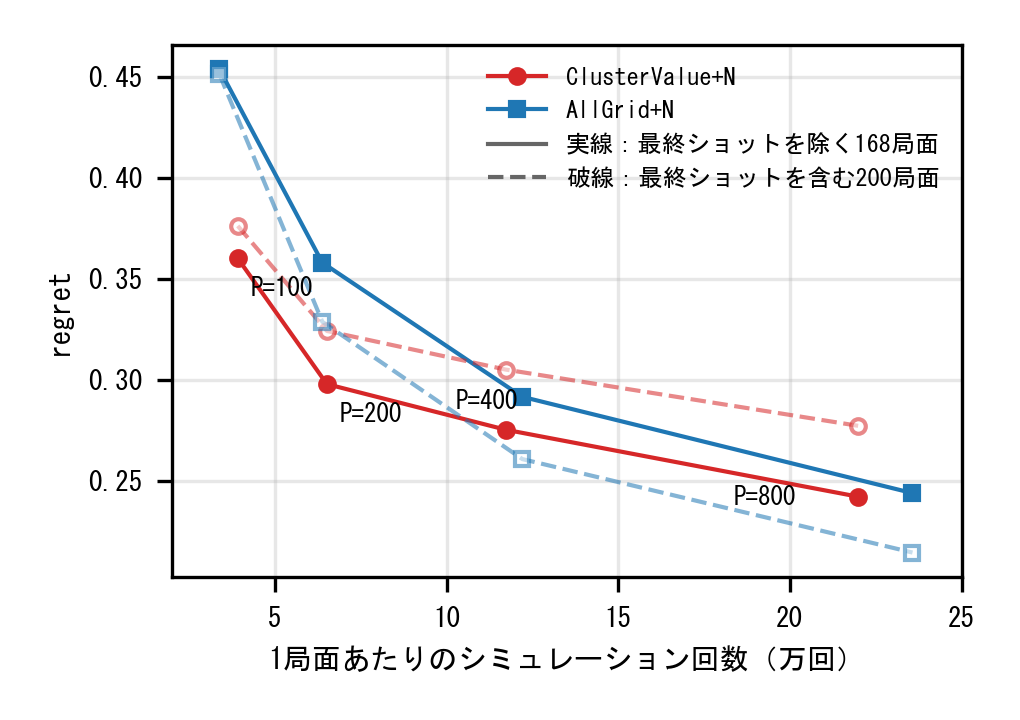
\includegraphics[width=\columnwidth]{figures/fig_budget.png}
\caption{プレイアウト予算$P$を変えたときのregret．実線は最終投を除く168局面，破線は最終投を含む200局面 (いずれも5シードの平均)．横軸は200局面での1局面あたりの物理シミュレーション回数の平均}
\ecaption{Regret versus the number of simulations for budgets $P=100$--$800$.}
\label{fig:budget}
\end{figure}

\subsubsection{代表手の選び方の影響}
\label{sec:res-repr}

子の数が同じ4個どうしで比べると，無作為に選ぶRandomK4+Nの0.552に対し，得点期待値で選ぶClusterValue+Nは0.309であった（$p=1\times10^{-43}$）．
一方，既存手法のmedoidによる選び方は，同じ数を無作為に選ぶRandomKと差がなかった
（外乱込み評価で0.396と0.383，決定的評価で0.488と0.491，いずれも$p>0.8$）．
結果盤面のクラスタで候補を分けても，その中からどの手を残すかを価値で決めなければ性能は上がらない．

既存手法との差がどのような局面で生じるかを，最良手（審判値が最大の手）が属するクラスタの大きさで局面を分けて調べた（\tabref{tab:csize}）．
最良手のクラスタが6〜10手の局面では，ClusterValue+NのregretがClusterMedoid+Nより0.090小さかった．
大きいクラスタほど，medoidが価値の低い手を代表に選ぶ機会が多いためである．
実際，審判値が最良から0.25以内の候補を含むクラスタについて，そのmedoid自体も最良から0.25以内である割合は45\%であった．
% 出典: gpw_experiment/cluster_vs_topk/paths_and_spaces_summary.txt (468局面)
一方，最良手のクラスタが1〜2手の局面では，ClusterMedoid+Nも最良手か，それと結果の近い手を代表として子に残すため差がない．
この層では，ClusterValue+NはAllGrid+Nよりregretが0.12〜0.13小さかった．
なお，最良手のクラスタの大きさは審判値を使って事後に分けたものであり，探索の時点で使える情報ではない．

\begin{table}[tb]
\caption{最良手のクラスタの大きさ別のregretの差 (ClusterValue+N $-$ 比較手法)．最終投を除く468局面．$^{**}p<0.01$，$^{*}p<0.05$ (層ごとのWilcoxon検定，補正なし)}
\ecaption{Regret difference by the size of the cluster containing the best move.}
\label{tab:csize}
\centering
\begin{tabular}{lrcc}\hline\hline
大きさ & 局面数 & 対ClusterMedoid+N & 対AllGrid+N \\\hline
1 & 40 & $+0.007$ & $-0.130^{**}$ \\
2 & 51 & $+0.007$ & $-0.117^{**}$ \\
3〜5 & 79 & $-0.056$ & $-0.061^{**}$ \\
6〜10 & 200 & $-0.090^{**}$ & $-0.028^{*}$ \\
11以上 & 98 & $-0.046$ & $+0.001$ \\\hline
\end{tabular}
\end{table}
% 出典: gpw_experiment/cluster_vs_topk/by_best_csize.txt

\subsection{実験のまとめ}
\label{sec:exp-summary}

\ref{sec:exp-purpose}節の3つの問いに対する結果をまとめる．
第一に，外乱込み評価はどの手法でもregretを下げ，その効果は主に木の損失の減少によるものであった．
第二に，候補を絞ることの利得は計算予算が小さいほど大きく，最終投を除けばどの予算でも提案手法は全探索を下回らなかった．
ただし最終投では，選別で最良手を落とすため全探索の方が良い．
第三に，得点期待値による代表手の選び方は無作為な選び方を大きく上回ったが，medoidによる選び方は無作為な選び方と変わらなかった．
以上から，提案手法の性能の向上は，得点期待値に基づく候補の選別と外乱込み評価によってもたらされたといえる．

%======================================================================
\section{考察}
\label{sec:discussion}
% 実験の説明がおわったあとのセクションでは、実験結果から導かれる考察について書いていく。今回のテーマだと軸は二つあって、一つは既存手法との差分を性能面で評価したらどうなったのかを明記すること。もう一つは、視覚的の評価が考えられるようになったということを示しましょう。具体的には、「人間にとって意味がある風にこの提案手法のクラスタリングはできるよ」ということが伝わるように書きたいです。この二つのサブセクションだけあれば十分です。ボロノイ領域との関係もここで提言しておきましょう。一つのサブセクション内に話をまとめれば十分だと思います。

\subsection{既存手法との性能の差}
\label{sec:disc-perf}

既存手法ClusterMedoidと提案手法は同じ結果盤面のクラスタを用いており，違いは代表手の選び方，採用するクラスタの数，評価の規約の3点である（\tabref{tab:diff}）．
同じ外乱込み評価の規約で比べると，提案手法のregretは既存手法より0.087（22\%）小さかった．
既存手法の代表手は価値を見ないため，約14個の子を持っても，同じ数を無作為に選ぶ場合と性能が変わらなかった．
これに対して提案手法は，クラスタ価値で4個のクラスタを選び，その中で推定値が最大の手を代表とすることで，
子の数を減らしながら有望な手を残している．
差が大きいのは最良手のクラスタが大きい局面であり（\tabref{tab:csize}），
大きなクラスタの中から盤面上の中心ではなく価値の高い手を選ぶことが，既存手法との差を生んでいる．
これは，先行研究~\cite{naka_gi58}で課題とした代表点の選び方と大きなクラスタの扱いに対する一つの解決である．
また，先行研究では全探索との一致率で評価していたが，等予算の全探索AllGrid+N自体のregretは0.334であり，
全探索の選択を正解とみなすことはできない．
審判値に基づくregretで評価したことで，提案手法が全探索を上回ることを示せた．

\subsection{人間にとって意味のあるクラスタ}
\label{sec:disc-visual}

提案手法のクラスタは，探索の単位であるだけでなく，人間が盤面を見て理解できる単位にもなる．
最終投を除く468局面では，1局面の候補は中央値59手で，中央値12個のクラスタに分かれた．
最大のクラスタは候補の約25\%を占め，クラスタの29\%は1手だけからなる．
2手以上のクラスタのうち38\%は種類の違う手（ドローとヒットなど）を含み，75\%は回転の違う手を含んでいた．
% 出典: gpw_experiment/paper_numbers/numbers.txt (A9P5N seed 42 の cluster_table)
すなわちクラスタは，ショットの名前や狙いではなく，投げた後にどのような盤面になるかで手をまとめている．
たとえば\figref{fig:cases}の局面1の15手からなるクラスタ（(b)の紫）は，ラベルの上ではドロー，相手の石に軽く当てる手，
フリーズ，ポストガードと異なるが，いずれも石を1個も出さず，投げた石がハウスの手前側に止まる手である．
% 出典: export_g9633_e1_s10 の cluster 0 (15手: 出た石なし, 投げた石のティーからの距離 0.53〜1.76m)

\begin{figure*}[t]
\centering
% 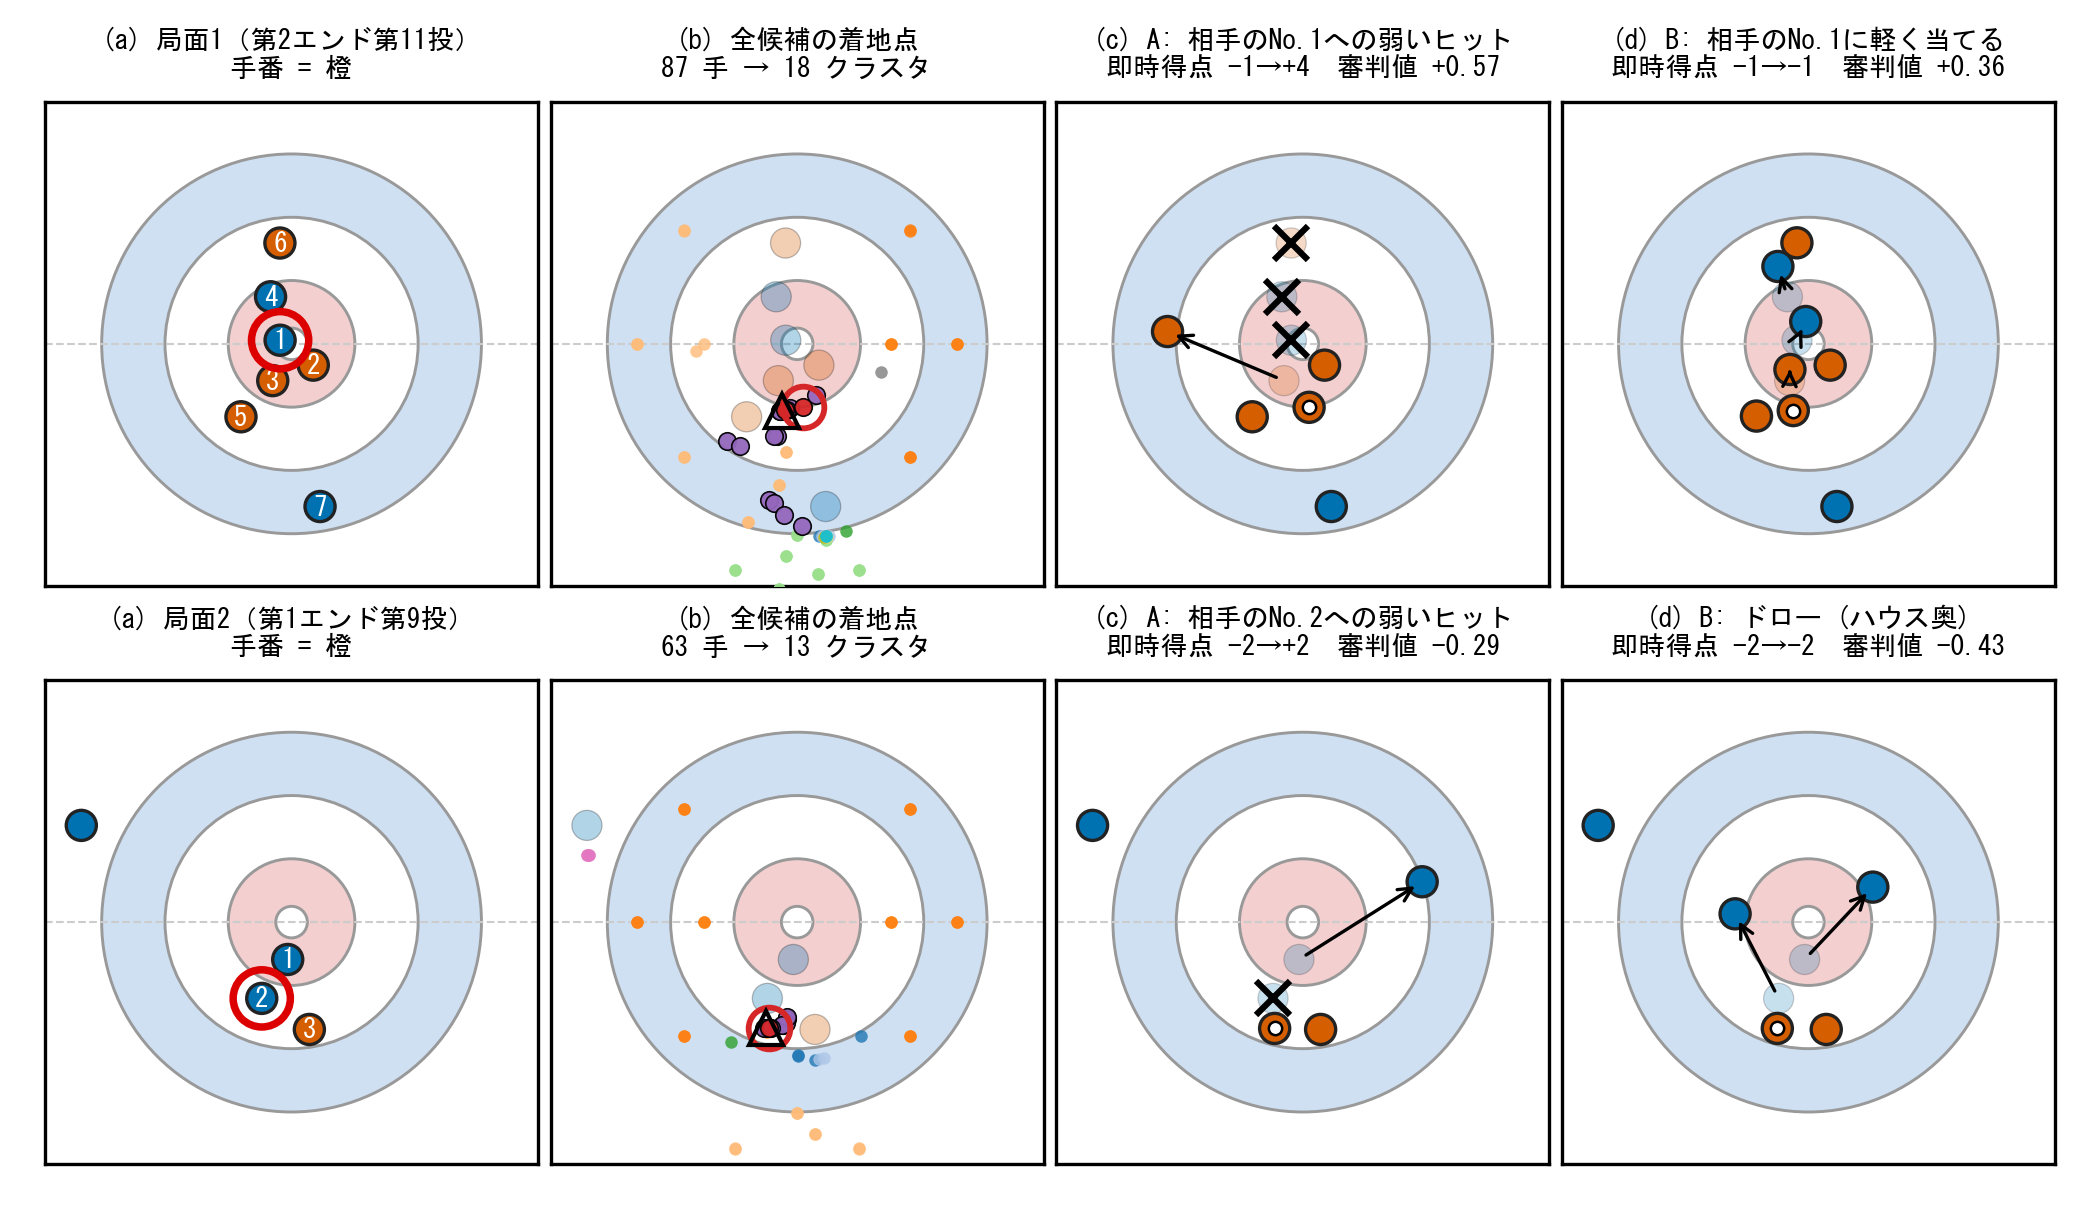
\includegraphics[width=\textwidth]{figures/fig_cases.png}
\caption{相手の中心の石を取り除く最良手の例 (上段：局面1，下段：局面2．どちらも手番は橙)．
(a) 局面 (石の数字はティーから近い順，赤丸は最良手が狙う石)．
(b) 全候補について投げた石が止まる位置．色はクラスタを表し，赤が最良手Aのクラスタ，紫が別の道Bのクラスタ，赤い円がA，△がB．プレーの外に出る石は描いていない．
(c) 最良手Aの結果盤面．(d) 別の道Bの結果盤面．矢印は動いた石，×はプレーの外に出た石，白点は投げた石を表す．
即時得点は投げた直後の盤面で数えた得点，審判値は手番側から見たエンドの得点の期待値}
\ecaption{Examples of best moves that remove the opponent's center stone.}
\label{fig:cases}
\end{figure*}
% 局面1 = g9633 e1 s10, 局面2 = g964 e0 s8 (図: scripts/plot_small_cluster_catalog.py --paper)

\figref{fig:cases}の2つの局面は，どちらも相手（青）がNo.1ストーンを持ち，手番の橙が負けている局面である．
局面1（第2エンド第11投）の最良手は，ティー上の相手のNo.1に弱く当てる手であり，その石と奥の相手の石がともにプレーの外に出て（奥の自分の石も1個出る），
投げた石がティーの手前に残る．
投げた直後の盤面で数えた得点（以下，即時得点）は$-1$から$+4$になり，審判値$+0.57$は全87手の中で最大である．
局面2（第1エンド第9投）の最良手は，相手のNo.1の手前にあるNo.2に弱く当てる手であり，
No.2がプレーの外に出ると同時にNo.1が奥へ押しやられ，投げた石がNo.2のあった位置の近くに残る．
即時得点は$-2$から$+2$になり，審判値$-0.29$は全63手の中で最大である．
% 出典: gpw_experiment/cluster_vs_topk/export/export_g964_e0_s8 (候補45: 相手 No.2 は除去, No.1 は 0.36m -> 1.21m)
2つの最良手は，いずれも相手の中心の石を取り除き，自分の石をティーの近くに残す手である．
これらの手の結果盤面は他のどの候補とも似ておらず，最良手のクラスタは局面1で2手，局面2で1手であった．
クラスタに分けると，こうした手は多数のドローやガードの変種に埋もれず，独立したまとまりとして現れる．
提案手法は，探索に使う4つの子にこれらの最良手を5シード中それぞれ2回と5回残し，regretは0.10と0.07であった
（AllGrid+Nは0.22と0.24，ClusterMedoid+Nは0.19と0.04）．
% 出典: gpw_experiment/cluster_vs_topk/catalog/index.csv (reg_A9P5N / reg_A1N / reg_A2N, 5seed平均)

このように最良手のクラスタが1〜2手の局面は，468局面中91局面（19\%）あり，石の多い局面では36\%（122局面中44局面）を占めた．
91局面の最良手のうち63手はヒットであり，相手の石を2個以上出す手が22手，レイズが18手あった．
% 出典: gpw_experiment/cluster_vs_topk/README.md (図カタログ: 最良手のクラスタが小さい 91 局面)
これらの局面では，提案手法の4つの子に最良手が残る割合が46\%（455回中208回）であり，それ以外の局面の14\%より高かった．
% 出典: gpw_experiment/paper_numbers/numbers.txt (6.3)
1手だけのクラスタはクラスタ価値が平均で薄まらないため，推定値の高い単独の手はそのまま採用されやすい．

クラスタは，即時得点は低いがエンド全体では同等に有利な別の道も示す．
\figref{fig:cases}(d)の手Bは，最良手とは別のクラスタに属し，即時得点は2点以上低いが審判値は最良に近い手である．
局面1のBは相手のNo.1に軽く当てる手で，即時得点は$-1$のままだが，審判値は$+0.36$（最良との差0.21）である．
局面2のBはハウスの奥を狙ったドローで，手前の石に当たって止まる．即時得点は$-2$のままだが，審判値は$-0.43$（差0.14）である．
局面2では，即時得点で2点を得る最良手Aでも，エンドの終わりまで考慮した期待値は$-0.29$にとどまる．
審判値が最良から0.25以内のクラスタを最良級クラスタと呼び，最良級クラスタのうち，その中で最良の手の即時得点が最大のものをA，
Aより即時得点が2点以上低い最良級クラスタをBと定義すると，AとBが別のクラスタに分かれる局面は468局面中184局面（39\%）あった．
Bの手はヒット77，ドロー73，ポストガード17，フリーズ15，プレガード2であった．
% 出典: gpw_experiment/cluster_vs_topk/paths_and_spaces_summary.txt
探索に使う4つの子がAとBを両方含む局面は7\%であったが，Bのクラスタのクラスタ価値の順位は中央値で12個中5位であり，
85\%の局面で上位8位以内に入った．
したがって別の道は，探索の子としてではなく，クラスタ価値の順に並べた結果盤面の一覧として人間に示すのが適している．
クラスタ価値は候補単位の推定値より審判値との順位相関が高い（200局面，決定的評価で中央値0.27から0.37，$p=4\times10^{-15}$）ため，
この一覧の順位は個々の候補の推定値の順位より信頼できる．
% 出典: E12 (run200, A9P5 決定的評価, R_pre=5)

\subsection{ボロノイ領域との関係}
\label{sec:disc-voronoi}

VOO~\cite{kim2020voot}は，評価済みの行動を母点として行動空間をボロノイ分割し，最良の母点のセルの中を重点的に探索する．
提案手法も，候補を領域に分けて各領域を1つの代表で扱い，推定値が最大の候補を含むクラスタを必ず採用する．
各候補を最も近い代表に割り当てた領域を，結果盤面の距離による一般化したボロノイ領域とみなせば，
提案手法はVOOと同様に最良の領域を重点的に探す方法と位置づけられる．
ただし距離$d$はベクトル空間の距離ではなく，平均連結法のクラスタは厳密にはボロノイ領域ではない．
両者の本質的な違いは，どの空間で近さを測るかにある．
そこで，VOOが前提とする「近い行動は近い価値を持つ」という性質が，行動空間と結果盤面の空間のどちらでよく成り立つかを調べた．

\begin{figure*}[t]
\centering
% 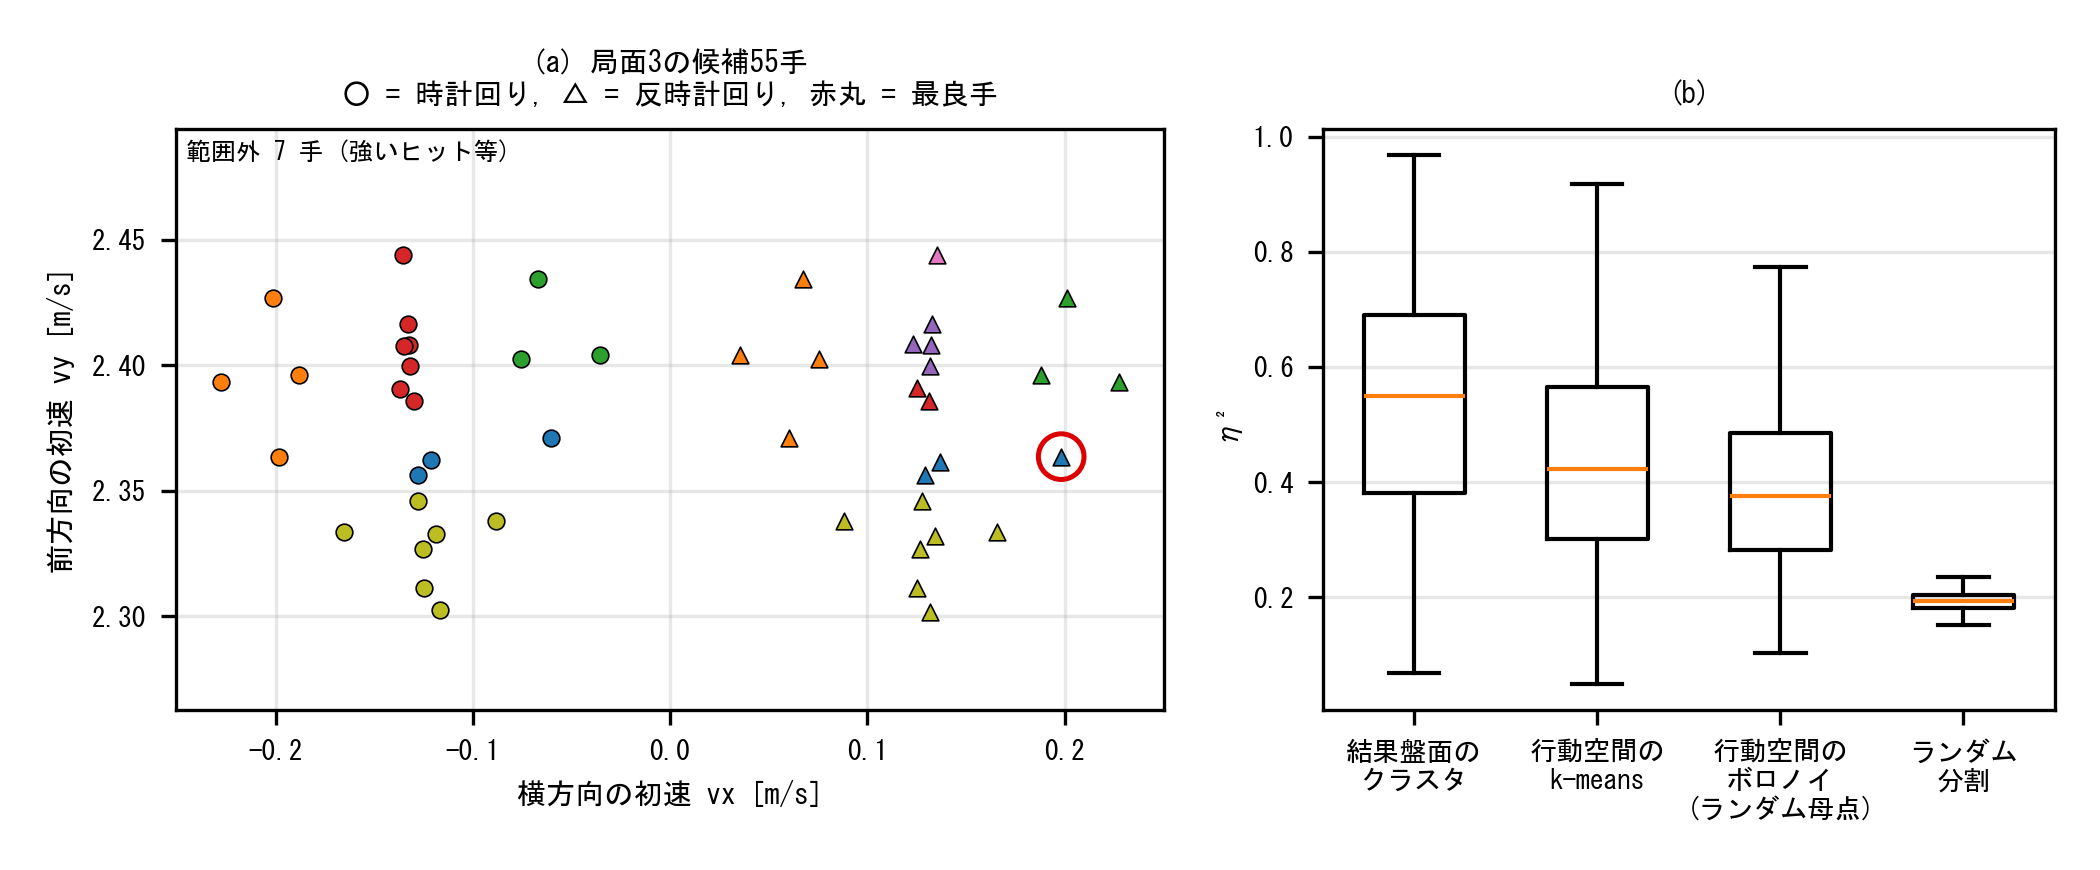
\includegraphics[width=\textwidth]{figures/fig_action_vs_result.png}
\caption{行動空間と結果盤面の空間．(a) 局面3 (第3エンド第4投) の候補を行動空間 (初速$v_x$，$v_y$) に置き，結果盤面のクラスタで色分けしたもの (価値の高い10クラスタに色を付けた．強いヒットなど7手は描画範囲外)．
(b) 最終投を除く468局面で，候補を同じ数の領域に分けたときの$\eta^2$ (審判値の分散のうち，領域の違いで説明される割合)}
\ecaption{Action space versus result space.}
\label{fig:space}
\end{figure*}
% 局面3 = g1555 e2 s3 (図: scripts/plot_action_vs_result_space.py)

行動空間は，初速$(v_x, v_y)$と回転方向の3次元とし，$v_x$と$v_y$は局面ごとに標準化し，回転の違いは1単位とした．
\figref{fig:space}(a)では，同じ狙いで強さだけが違う手（縦に並ぶ点）が別のクラスタに分かれ，回転の違う手（○と△）が同じクラスタに入っている．
468局面では，行動空間で最も近い候補が別のクラスタに属する割合は中央値で45\%であった．
最も近い候補との審判値の差の中央値は，行動空間では0.140，結果盤面の距離では0.130であり，
結果盤面で近い候補の方が価値も近かった（$p=6\times10^{-15}$）．
% 出典: gpw_experiment/cluster_vs_topk/paths_and_spaces_summary.txt (局面ごとの値の中央値; Wilcoxon)
さらに，候補を同じ数の領域に分けたときの$\eta^2$を比べると（\figref{fig:space}(b)），結果盤面のクラスタは中央値0.549であり，
行動空間のk-means（0.422）と，候補から無作為に選んだ母点による行動空間のボロノイ分割（VOOのセルに相当，20回の平均，0.375）のいずれよりも大きかった
（それぞれ$p=2\times10^{-28}$，$p=3\times10^{-55}$）．
k-meansで$v_x$，$v_y$を四分位範囲で割って尺度を合わせた場合も0.393であった．
1手だけのクラスタが多いことによる効果を除くため，クラスタと同じ大きさの領域に無作為に分けた場合を対照としたが，その値は0.193であった．
% 出典: gpw_experiment/cluster_vs_topk/paths_and_spaces_summary.txt, scripts/analyze_paths_and_spaces.py

以上から，VOOTが前提とする「近い行動は近い価値を持つ」という性質は，カーリングでは行動空間より結果盤面の空間でよく成り立つ．
狙いがわずかに違うだけで石に当たるかどうかが変わる一方，離れた行動が同じ結果を生むためである．
結果盤面のクラスタは価値のまとまった領域であり，探索で価値を推定する単位としても，人間に示す単位としても適している．

%======================================================================
\section{今後の課題}
\label{sec:future}
% ここでは、考察というより、今後の課題について書いていきます。実験結果から分かることや、今の提案手法の弱みを明記し、それをどのように改善したいのかを書く。

実験から，提案手法には次の弱みがあることが分かった．
第一に，エンドの最終投では，事前推定による選別で得点につながる少数の手を落とし，全探索より性能が下がる（\ref{sec:res-budget}節）．
最終投の局面だけ全探索に切り替えると，$P=200$の500局面全体のregretは計算上約0.02下がる．
% 出典: 0.287 x 32 / 500 = 0.018 (E14 層別 r=1)
第二に，計算予算が大きくなると全探索との差はなくなる．
提案手法の利点は予算が小さい場合に限られるため，持ち時間に応じて選別の強さを変える方法を検討する必要がある．
第三に，得点期待値に基づく選別はルートノードだけに適用しており，深さ1以降のノードでは既存手法の規則を用いている．
事前推定のコストを抑えながら，内部のノードにも価値に基づく選別を広げることが課題である．
第四に，本論文の比較はシミュレーション回数を揃えたものであり，距離の計算やクラスタリングの時間を含まない．
持ち時間のある実際の対戦で評価する必要がある．

視覚的評価については，クラスタが結果の種類で手をまとめることを盤面の図と統計で示したが，
人間がこの提示によって良い手や別の道に気付けるかは確かめていない．
カーリングの経験者による評価が今後の課題である．
また，\ref{sec:disc-voronoi}節の結果から，VOOが最良のセルの中で新たな行動を生成するのと同様に，
有望なクラスタの結果を生む行動の周辺で新たな候補を生成することが考えられる．
距離関数の重みは先行研究~\cite{naka_gi58}で人手で調整した値のままであり，その調整も残されている．

%======================================================================
\section{おわりに}
\label{sec:conclusion}
% このセクションでは全体の論文の概要を取りまとめます。このセクションで書かれていることは、"はじめに"のセクションで示された内容と論理的に一貫するように全体のまとめについて書くので、そこまで長い文章になる必要は無いです。600文字程度で収まるといいです。

本論文では，デジタルカーリングのMCTSにおける候補手の削減について，結果盤面のクラスタを保ったまま，
クラスタの採用と代表手の選出に得点期待値を用いるClusterValueと，外乱込み評価を組み合わせた手法を提案した．
審判値に基づくregretで500局面を等予算で比較した結果，提案手法は既存手法ClusterMedoidよりregretが22\%小さく，候補を絞らない全探索も上回った．
その利得は計算予算が小さいほど大きく，最終投を除けば全探索の約5〜6割の計算量で同程度の品質が得られた．
性能の向上は，得点期待値に基づく選別と外乱込み評価によるものであり，medoidによる代表手の選び方は無作為な選び方と変わらなかった．
また，結果盤面のクラスタは手を結果の種類でまとめ，相手の中心の石を取り除くような他と似ていない最良手や，
即時の得点は低いがエンド全体では同等に有利な別の道を，独立したまとまりとして示せることを確認した．
結果盤面による分割は，VOOTのような行動空間の分割よりも価値のまとまった領域を作った．
今後は，最終投での選別の改善と，持ち時間のある対戦および人間による評価を進める．


%======================================================================
% 1段幅の図の例 (位置指定に h は使わない)
%\begin{figure}[tb]
%  \centering
%  \includegraphics[width=\columnwidth]{figures/xxx.pdf}
%  \caption{和文見出し}
%  \ecaption{English caption.}
%  \label{fig:xxx}
%\end{figure}
%
% 2段幅の図の例 (位置指定は t のみ)
%\begin{figure*}[t]
%  \centering
%  \includegraphics[width=\textwidth]{figures/yyy.pdf}
%  \caption{和文見出し}
%  \ecaption{English caption.}
%  \label{fig:yyy}
%\end{figure*}
%
% 表の例 (見出しは表の上, 一番上の罫線は二重線, 左右端に縦罫線なし)
%\begin{table}[tb]
%  \caption{和文見出し}
%  \ecaption{English caption.}
%  \label{tab:zzz}
%  \centering
%  \begin{tabular}{lcc}\hline\hline
%    手法 & 列1 & 列2 \\\hline
%    A & -- & -- \\
%    B & -- & -- \\\hline
%  \end{tabular}
%\end{table}
% 参照は \figref{fig:xxx}, \tabref{tab:zzz}

%======================================================================
%\begin{acknowledgment}
%謝辞．
%\end{acknowledgment}

% 本文で \cite していない文献はリストに出ない
\bibliographystyle{ipsjunsrt}
\bibliography{references}

%\appendix
%\section{付録の節}

\end{document}
